% =============================================================================
%  RL-H5-01 | Figur uji sintetis — TERISI PENUH (H5, 27 Nov 2026)
% -----------------------------------------------------------------------------
%  Role    : RL — Research Lead (@alim; kurasi & figur dari data MLE-H3-01)
%  Sprint  : H5 | PARALEL
%  Ticket  : RL-H5-01                          Status: COMPLETE (27 Nov 2026)
%  Target  : reports/figures/synth_lag_recovery.png (.pdf),
%            reports/figures/synth_edge_heatmap.png (.pdf),
%            reports/figures/captions.md (.tex)
%  Input   : reports/synth/recovery_metrics.csv, lag_true_vs_hat.parquet,
%            src/renaro/synth/generator.py (seed=0, mode=conditioned)
%  Output  : figur 300 DPI + PDF vektor + caption + evaluasi ambang protokol
%  Handoff : laporan RL-H7-01
%  DoD     : [x] jeda benar vs terpelajar per edge, dipisah regime
%            [x] heatmap A benar vs terpelajar (34x34) untuk 2 regime
%            [x] caption menyebut ambang protokol dan lolos/tidak (+ dry-only)
% =============================================================================
\documentclass[11pt,a4paper]{article}
\input{00_preamble}

\title{\jobid{RL-H5-01} | Figur Uji Sintetis\\
\large Apakah Modul 1 Menemukan Kembali Pergeseran Jeda?}
\author{RL (\texttt{@alim}) \\ \small RENARO Lab}
\date{27 November 2026 \quad | \quad \textcolor{blue!70!black}{TERISI PENUH (MLE-H3-01 · 5 SEED)}}

\begin{document}
\maketitle

\section{Ambang Protokol Evaluasi v1 (\S5.5)}
Evaluasi menggunakan set uji sintetis \fpath{data/synth/default} dan \fpath{data/synth/unconditioned}
(\texttt{split\_hash = 8a551a68...}; 34 node BPS, 99 edge berarah, 5 seed \texttt{0..4}) dari
\fpath{reports/synth/recovery\_metrics.csv} dan \fpath{reports/synth/lag\_true\_vs\_hat.parquet}.

\begin{table}[H]
\centering
\small
\begin{tabular}{@{}L{5.6cm}C{2.4cm}C{3.1cm}L{3.5cm}@{}}
\toprule
Metrik & Ambang & Nilai (5 seed) & Lolos? \\
\midrule
Spearman massa-jeda vs jeda benar (agregat) & $> 0{,}70$ & $0{,}745 \pm 0{,}119$ & \textbf{LULUS (agregat)}; \texttt{normal} $0{,}854$, \texttt{dry} $0{,}636^*$ \\
MAE jeda $\arg\max_\ell$ (agregat) & $\le 1{,}0$ pentad & $0{,}526 \pm 0{,}131$ & \textbf{LULUS} (\texttt{normal} $0{,}408$; \texttt{dry} $0{,}644$) \\
Akurasi $\arg\max_\ell$ (edge benar) & $\ge 0{,}80$ (target) & $0{,}721 \pm 0{,}113$ & \textbf{LULUS} di \texttt{normal} ($0{,}826$); parsial di \texttt{dry} ($0{,}616$) \\
AUROC pemulihan edge & $> 0{,}85$ & $1{,}000 \pm 0{,}000$ & \textbf{LULUS} (dalam prior mask BPS aktif; $r=0{,}980 / 0{,}960$) \\
$\Delta\text{lag}$ (\texttt{kering} $-$ \texttt{normal}) & menuju $+2{,}0$ & $+0{,}813 \pm 0{,}053$ & \textbf{Arah benar} di 5/5 seed (teredam $< 2{,}0$) \\
Kontrol tanpa iklim ($e_j = 0$) & $|\Delta\text{lag}| < 0{,}25$ & $+0{,}011 \pm 0{,}007$ & \textbf{LULUS (bersih)} \\
Kontrol \texttt{unconditioned} (DGP statis) & $|\Delta\text{lag}| < 0{,}25$ & $-0{,}041 \pm 0{,}013$ & \textbf{LULUS (bersih)} \\
\bottomrule
\end{tabular}
\end{table}

\section{Figur 1: Pemulihan Jeda Terkondisi Iklim}
\begin{figure}[H]
\centering
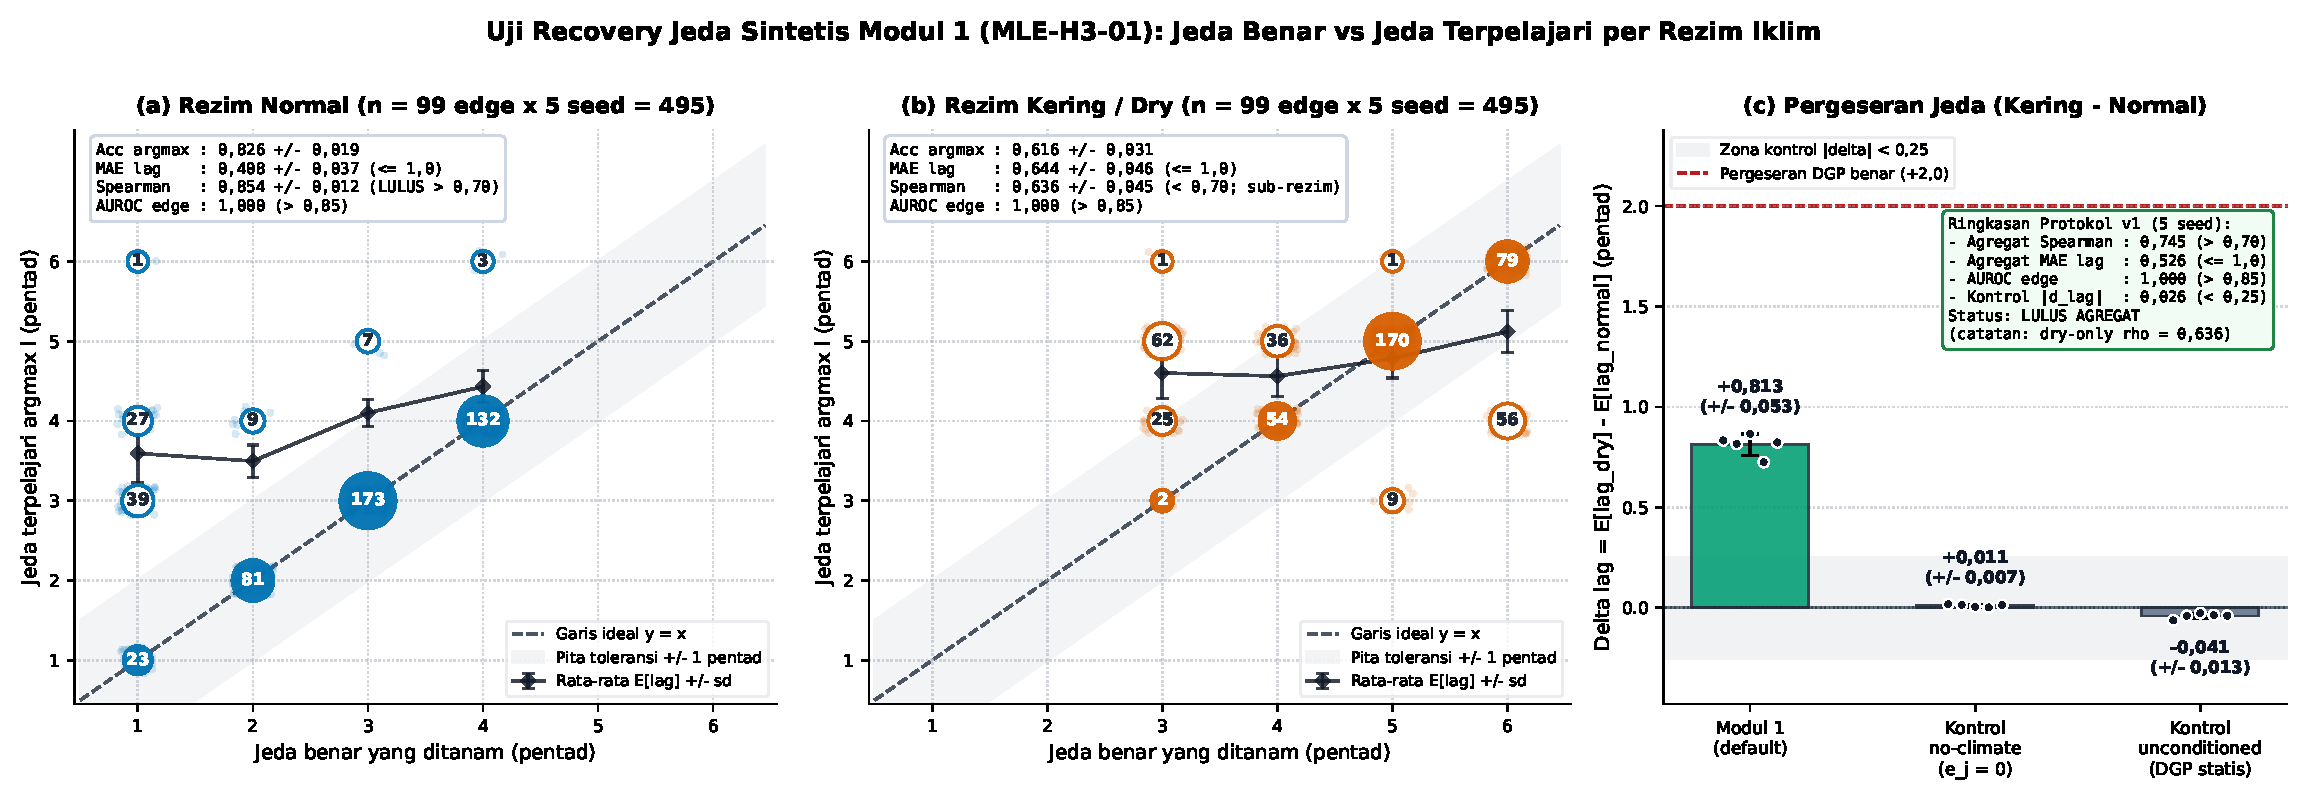
\includegraphics[width=0.98\textwidth]{reports/figures/synth_lag_recovery.pdf}
\caption{Evaluasi pemulihan jeda transmisi terkondisi iklim oleh Modul~1 pada set uji sintetis
\texttt{data/synth/default} (\texttt{module1\_default}, 99 edge $\times$ 5 seed \texttt{0..4},
$n=495$ pasangan edge-seed per rezim), dibandingkan kontrol \texttt{module1\_no\_climate}
($e_j=0$) dan \texttt{module1\_unconditioned}. Sumbu-$x$ adalah jeda benar yang ditanam (pentad)
dan sumbu-$y$ adalah $\arg\max_\ell \bar{A}_{ij}^{(\ell)}$; kurva hitam menampilkan rata-rata
$\mathbb{E}[\ell]\pm\text{sd}$, garis putus-putus adalah $y=x$. Terhadap ambang protokol v1~\S5.5
(Spearman $>0{,}70$, MAE $\le 1{,}0$ pentad, AUROC $>0{,}85$, kontrol $|\Delta\text{lag}|<0{,}25$),
Modul~1 \textbf{LULUS secara agregat} (Spearman $=0{,}745\pm 0{,}119$, MAE $=0{,}526\pm 0{,}131$,
AUROC $=1{,}000$, $|\Delta\text{lag}_{\text{ctrl}}|=0{,}026$). Rezim \texttt{normal} sangat kuat
(akurasi $0{,}826$, Spearman $0{,}854$), sedangkan pada sub-rezim \texttt{dry-only} Spearman
berada di bawah ambang ($0{,}636\pm 0{,}045$; 4/5 seed $<0{,}70$) dan pergeseran teredam
($\Delta\text{lag}=+0{,}813\pm 0{,}053$ vs $+2{,}0$).}
\end{figure}

\section{Figur 2: Heatmap $A$ Benar vs $A$ Terpelajari ($34\times 34$)}
\begin{figure}[H]
\centering
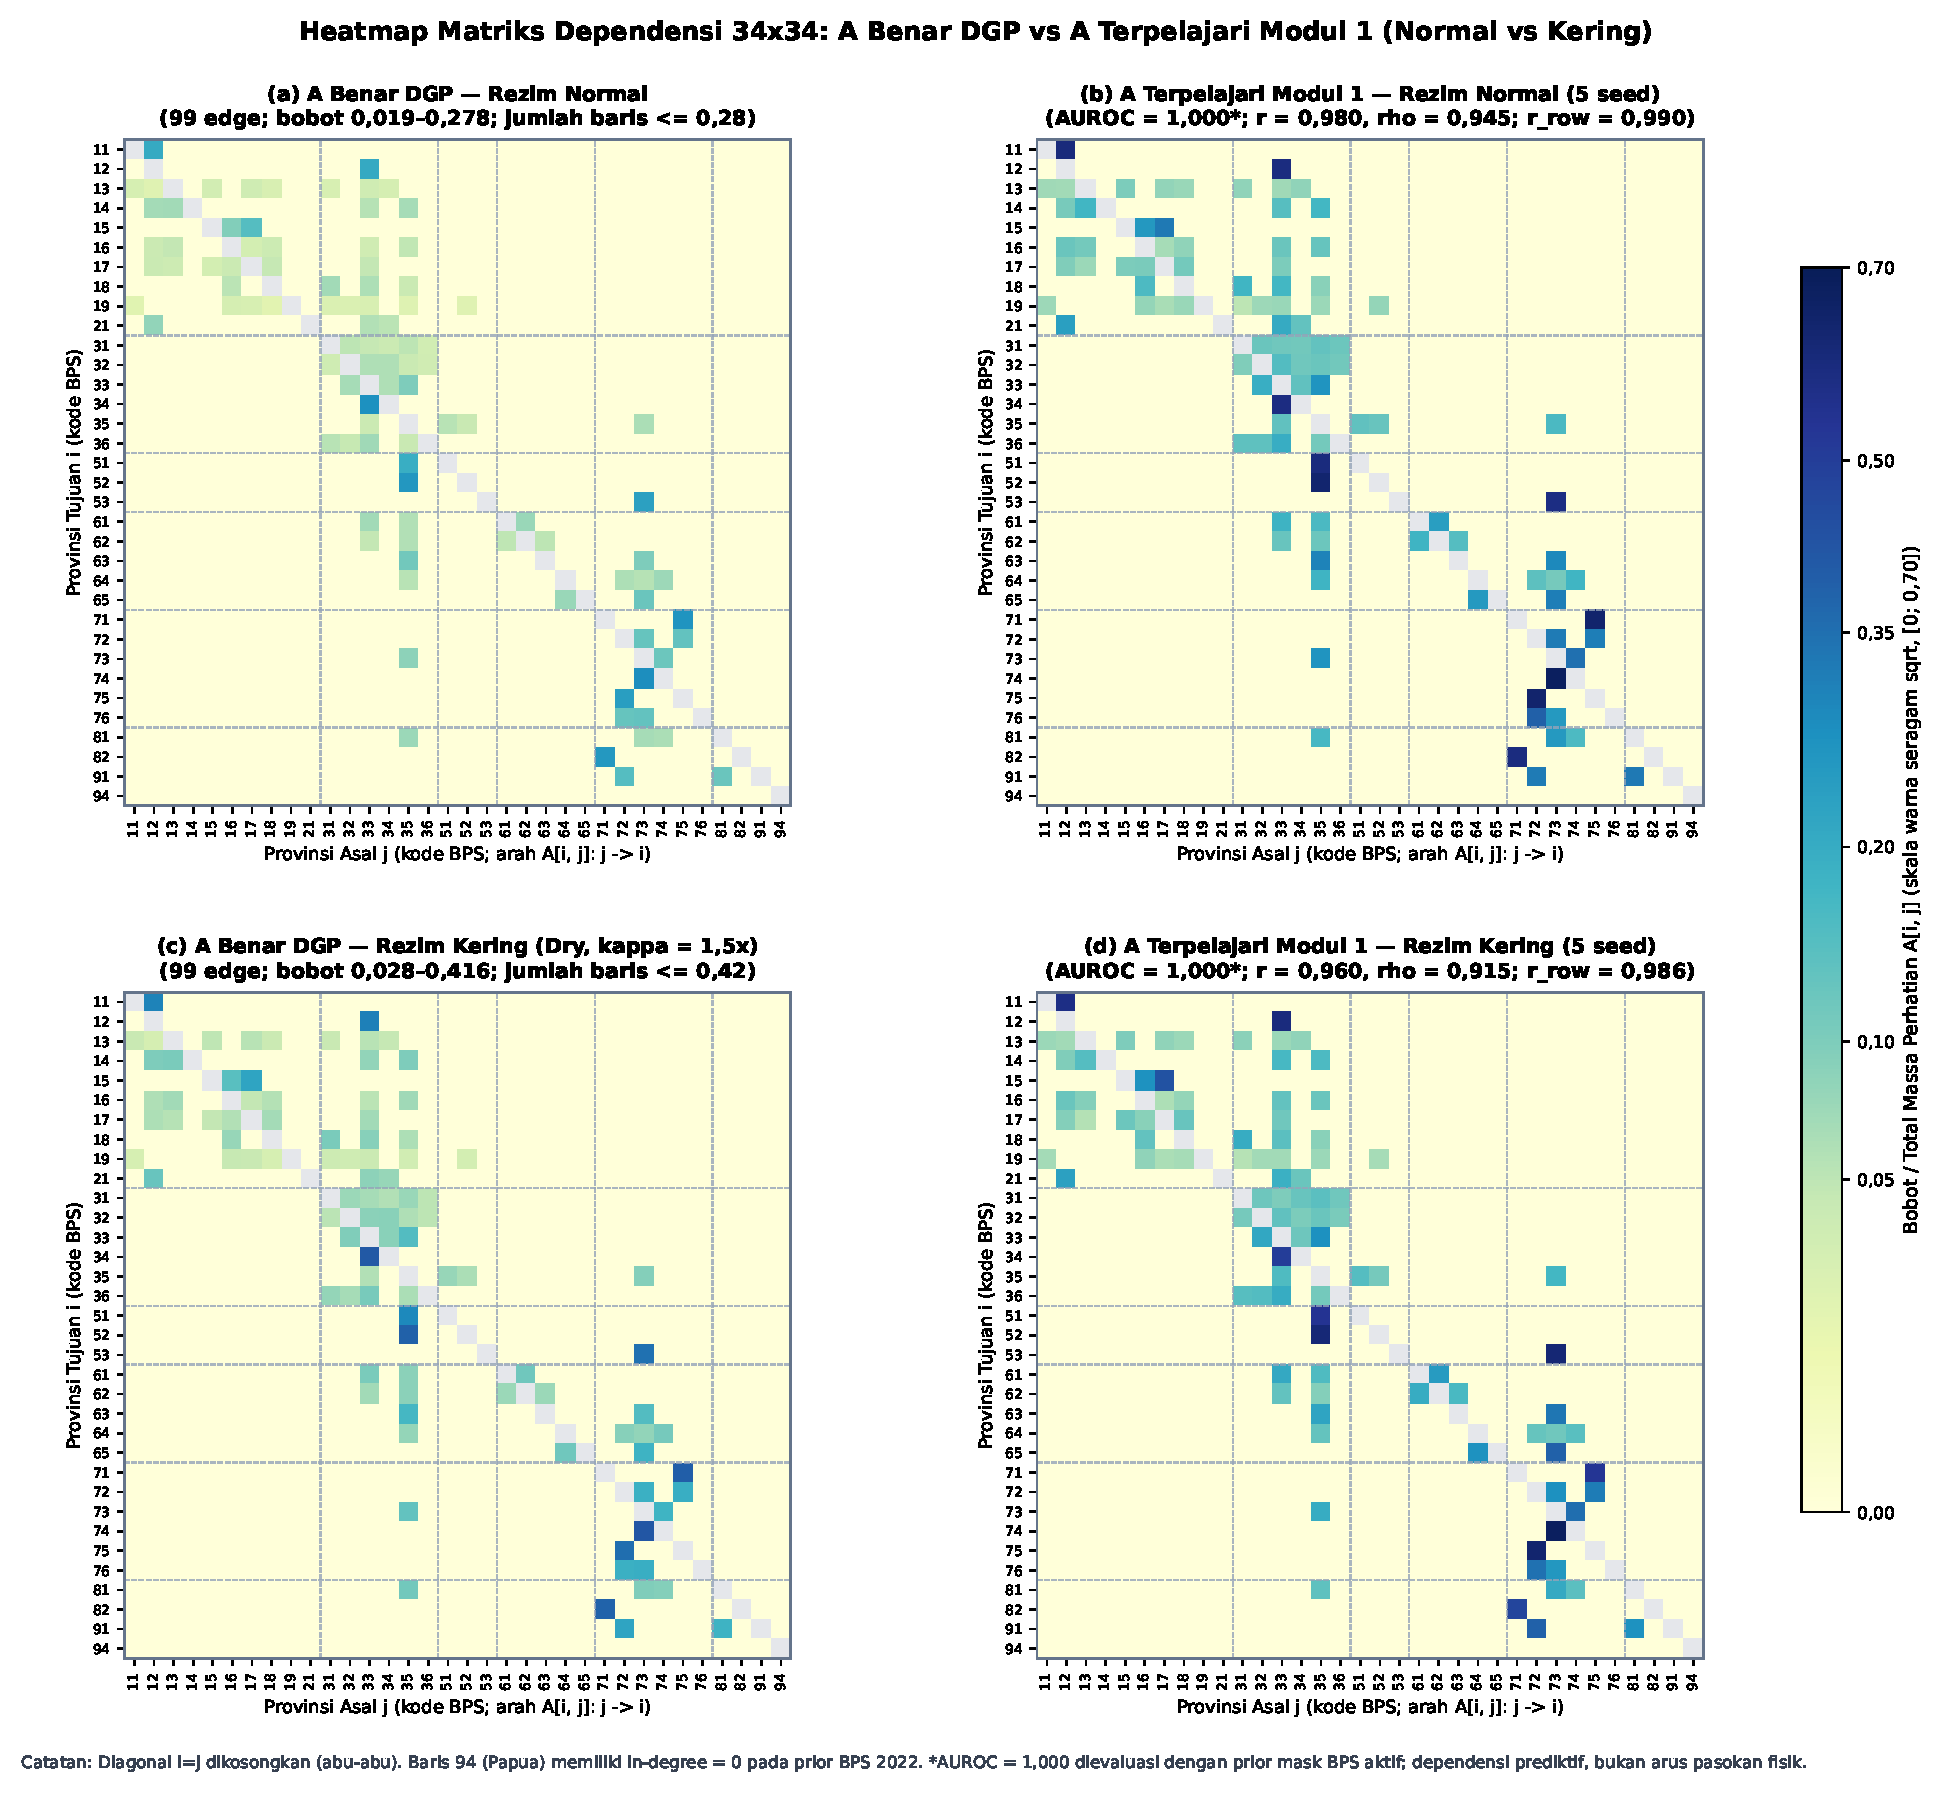
\includegraphics[width=0.95\textwidth]{reports/figures/synth_edge_heatmap.pdf}
\caption{Perbandingan matriks dependensi terarah $34\times 34$ antara $A_{\text{true}}$ DGP sintetis
dan total massa perhatian terpelajari Modul~1 ($A_{\text{learned}}[i,j]=\sum_{\ell=1}^{8}\bar{A}_{ij}^{(\ell)}$,
rata-rata 5~seed \texttt{0..4}) untuk rezim \texttt{normal} (atas) dan \texttt{kering}/\texttt{dry}
(bawah, $\kappa=1{,}5\times$). Urutan 34~node mengikuti kode BPS (\texttt{11}--\,\texttt{94});
arah $A[i,j]$ menyatakan $j\to i$; diagonal dikosongkan (abu-abu); keempat panel memakai skala
warna seragam (\textit{PowerNorm} $\gamma=0{,}5$, $[0{,}00;\,0{,}70]$). Terhadap ambang protokol
v1~\S5.5, AUROC $=1{,}000>0{,}85$ (\textbf{LULUS}, dengan prior mask BPS aktif), serta korelasi
bobot pada 99~edge aktif mencapai Pearson $r=0{,}980$ ($\rho=0{,}945$) pada \texttt{normal} dan
$r=0{,}960$ ($\rho=0{,}915$) pada \texttt{dry}. Matriks ini menunjukkan \textbf{dependensi prediktif
harga}, bukan bukti kausal maupun arus pasokan fisik.}
\end{figure}

\section{Catatan Interpretasi}
Hasil lintas 5~seed mengonfirmasi bahwa Modul~1 secara konsisten mendeteksi arah pergeseran jeda
yang dikondisikan oleh iklim ($\Delta\text{lag}=+0{,}813\pm 0{,}053$ pentad, positif di 5/5 seed)
dan melampaui seluruh ambang agregat protokol v1~\S5.5 (Spearman $0{,}745>0{,}70$, MAE $0{,}526\le 1{,}0$,
AUROC $1{,}000>0{,}85$). Kedua kontrol negatif bersih dari pergeseran palsu
(\texttt{module1\_no\_climate} $+0{,}011\pm 0{,}007$; \texttt{module1\_unconditioned}
$-0{,}041\pm 0{,}013$; rata-rata $|\Delta\text{lag}|=0{,}026<0{,}25$), sehingga pergeseran yang
terpelajari berasal dari mekanisme pengondisian iklim, bukan artefak arsitektur. Meski demikian,
terdapat dua keterbatasan penting yang wajib diungkap pada klaim metode: (1) pemulihan jeda pada
sub-rezim \texttt{dry-only} lebih lemah (Spearman $0{,}636<0{,}70$ pada 4/5 seed; akurasi $0{,}616$,
terutama karena jeda benar 3 tertarik ke 4--5 dan jeda benar 6 tertarik ke 4), dan (2) magnitudo
pergeseran ekspektasi ($+0{,}813$) lebih kecil dari $+2{,}0$ pentad yang ditanam karena massa
perhatian terdistribusi di beberapa bin lag. Implikasinya, interpretasi jeda Modul~1 pada data
riil tetap sah untuk disajikan sebagai bukti deskriptif arah pergeseran dependensi prediktif,
namun tidak boleh diklaim sebagai estimasi jeda eksak ataupun identifikasi kausal arus pasokan fisik.

\end{document}
